\documentclass[MSc,english]{Container/thesistemplate}
\usepackage[Lenny]{fncychap}
\usepackage[nottoc]{tocbibind}
\usepackage{wrapfig}

\begin{document}

\author{Federico Vincenzo Mastellone}
\title{Understanding oscillopathies in the Cortico-Basal Ganglia-Thalamocortical loop: an approarch with three heterogeneous populations of Kuramoto oscillators}
\aayear{2021/2022}

\begin{supervisors}
   \supervisor{}{Prof.}{E. Cataldo}
\end{supervisors}

\begin{cosupervisors}
   \cosupervisor{}{Prof.}{A. Mazzoni}
\end{cosupervisors}

\maketitlepage

\tableofcontents

\chapter*{Introduction}
\addcontentsline{toc}{chapter}{Introduction}


\chapter{Background}
\section{The Basal Ganglia Complex}
Among the various complex structures one can find in a mammal's brain the Basal Ganglia \textbf{(BG)} is one of those whose basic anatomy and connectivity hasn't ran into much change in half a billion years \cite{evol} \cite{nelsonkreitzer}.
\\ It is located at the base of the forebrain and it consists of several nuclei; these nuclei form a highly \emph{non linear network} so that each nucleus projects, somehow, to itself and the others. Some of these nuclei also project and receive projections from structures outside the BG --- the \emph{Striatum} and the \emph{Globus Pallidus} are an example, being connected to the \emph{Thalamus} and the \emph{motor Cortex}.
\\ One question rapidly arises: \emph{why had this complex been preserved during evolution? What is its purpose?}
\\ The BG are principally involved in the selection and implementation of purposeful actions in response to external and internal cues. This means that this structure is involved in those tasks in which a facilitation or a suppression of a movement is required. On top of that, it is involved in a series of fundamental non-motor behaviours such as: \emph{emotions}, \emph{language}, \emph{procedural learning} and last but not least \emph{decision making} \cite{simonyan}. It is worth adding that \emph{Dopamine} --- a \emph{neurotransmitter} which is involved in the processing of reward after the completion of a task --- is produced in the BG and plays a crucial role in controlling motor functions and in learning new motor skills.

\subsection{Anatomy}
From a general point of view, the BG complex --- such as any complex in the brain --- consists of some input nuclei, some output nuclei and some internal nuclei whose role is that to process the signals incoming in the input nuclei.
\\ Briefly, this is the list of nuclei composing the Basal Ganglia:

\begin{itemize}
    \item The \emph{Striatum} $\longleftrightarrow$ \textbf{(Str)}, which is formed by 
    \begin{enumerate}
        \item \emph{Putamen}
        \item \emph{Caudate nucleus}
    \end{enumerate}
    
    \item The \emph{Globus Pallidus}, generally divided into
    \begin{enumerate}
        \item the \emph{internal} part $\longleftrightarrow$ \textbf{(GPi)}
        \item the \emph{external} part $\longleftrightarrow$ \textbf{(GPe)}
    \end{enumerate}
    
    \item The \emph{Substantia Nigra}, consisting of
    \begin{enumerate}
        \item its \emph{Pars Compacta} $\longleftrightarrow$ \textbf{(SNc)}
        \item its \emph{Pars Reticulata} $\longleftrightarrow$ \textbf{(SNr)}
    \end{enumerate}
    
    \item The \emph{Subthalamic Nucleus} $\longleftrightarrow$ \textbf{(STN)}
\end{itemize}

\begin{figure}[ht!]
  \centering
    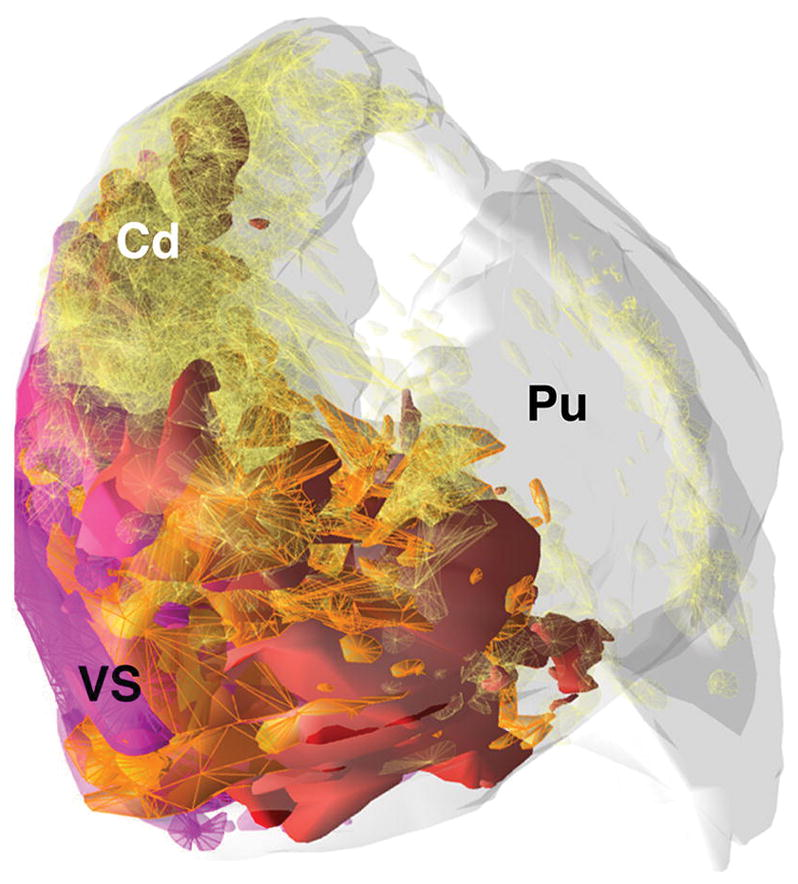
\includegraphics[scale=.8]{Images/striatumrec.jpg}
    \caption{Three dimensional reconstruction of the Striatum including the \emph{Caudate} \textbf{(CD)}, the \emph{Putamen} \textbf{(PD)} and the \emph{Ventral Striatum} \textbf{(VS)}. (Figure adapted from \cite{striatalfigure}).}
\end{figure}

\subsection*{Input nuclei}
The \textbf{Striatum} is the major input structure of the Basal Ganglia receiving projection from the Thalamus and pretty much every cortical area. These cortical areas can be grouped into regions each related to a different function: \emph{sensorimotor}, \emph{cognitive} and \emph{affective}; each of these sends excitatory projections to subregions of the Striatum forming distinct channels. There is evidence pointing out that these channels are overlapping and this may serve an integrative function between cognitive, motor and limbic signals deriving from cortical areas. 
\\  Excitatory projections from the Thalamus are topographically organized and overlapping in a similar fashion as the cortico-striatal projections. \cite{nelsonkreitzer}.
\\ In addition to the inputs received from areas outside the Basal Ganglia, the Striatum also collects projections from the SNc and the \emph{Ventral Tegmental Area} \textbf{(VTA)}; these afferent are extremely important since the main neurotransmitter released in the synaptic cleft is \emph{dopamine}. 

\begin{figure}[ht!]
    \centering
    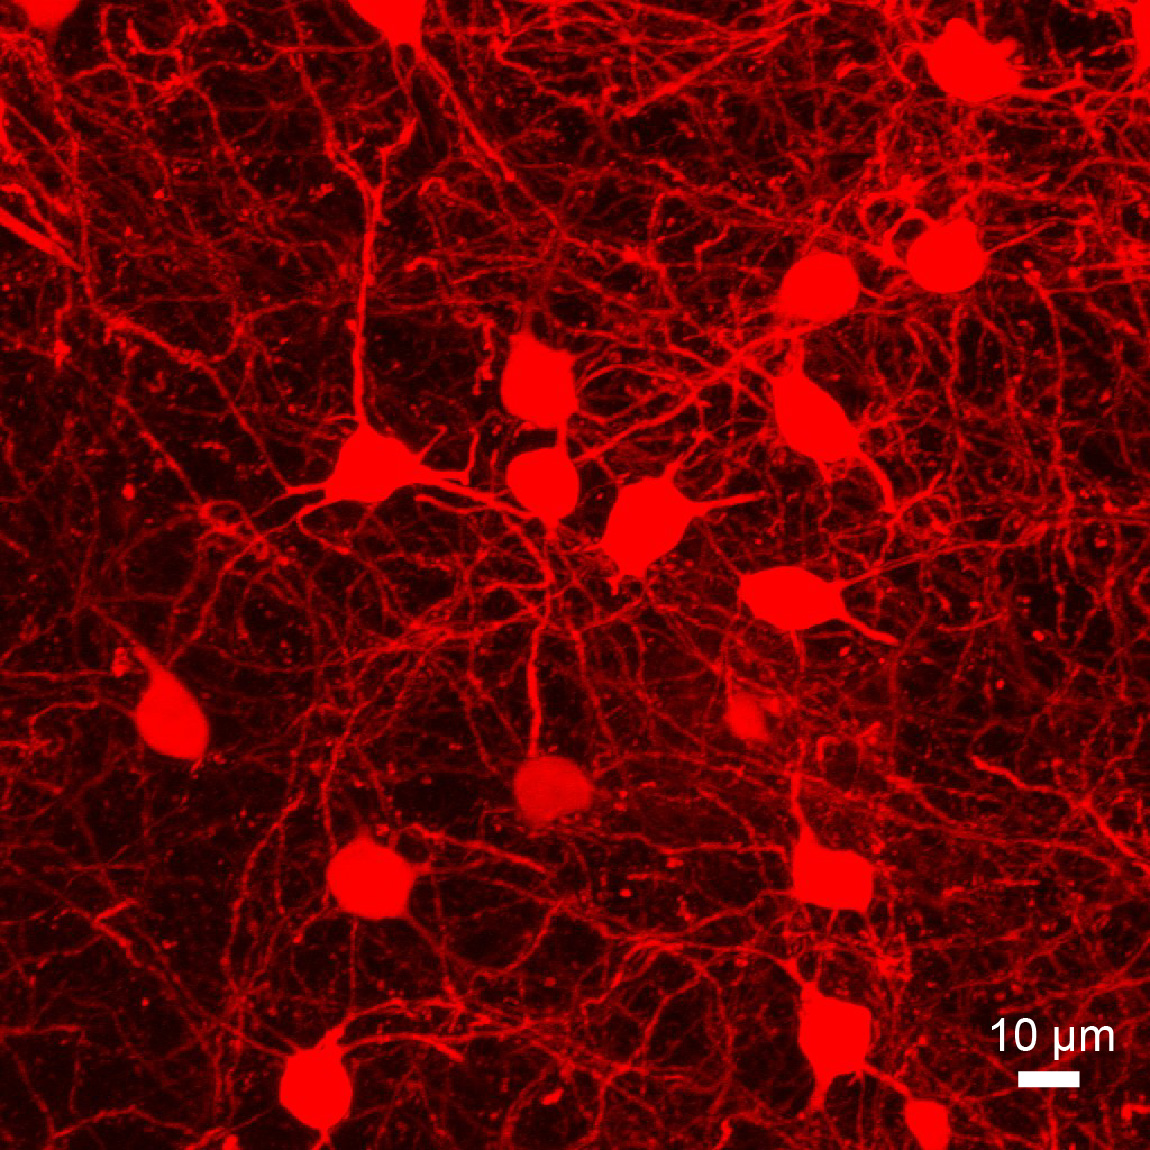
\includegraphics{Images/MediumSpinyNeurons.jpg}
    \caption{Confocal microscopy Z projection of medium spiny neurons (MSNs) in the mouse striatum.}
    \label{fig:msn}
\end{figure}

Among the total number of neurons in this structure, $N_{Str}=(2,791\pm 188)\cdot 10^3$ \cite{oorschot}, 95\% of them are \emph{Medium Spiny Neurons} \textbf{(MSNs)} (Fig.\ref{fig:msn}), a type of GABAergic inhibitory neuron, which can be divided in those having the D1-type dopamine receptors and those having the D2-type dopamine receptors; the difference consists in the chemical processes deriving from the \emph{neurotransmitter-receptor} bound. D1 receptors initiates a second messenger-signaling cascade resulting in the depolarization of the post-synaptic MSN, while the same process results in the hyperpolarization of the post-synaptic MSN having the D2 receptor \cite{utterbasso}. Hence, the role of D1 receptors is to enhance cortico-striatal influence and this is in contrast to the reduction mediated by D2 receptors.
\\ Approximately half of the MSNs projects directly to the SNr or the GPi while the remaining half points to the GPe. Dopamine has thus a remarkable influence on the processing of the signals incoming from the Cortex and travelling towards the other BG nuclei.
\\ The other input nucleus in the BG is the \textbf{Subthalamic Nucleus} which, as the name suggests, is positioned just under the Thalamus and it's composed primarily of \emph{glutamatergic neurons}, $N_{STN} = (13.56\pm 1.41)\cdot 10^3$ \cite{oorschot}. As the Striatum the STN receives projections from the \emph{Primary Motor Cortex}, the \emph{Supplementary Motor Cortex} and the \emph{Premotor Cortex} but in a smaller amount. Also, it has afferents coming from the GPe. The STN is the \emph{only} nucleus in the \emph{whole} Basal Ganglia complex to \emph{send excitatory projections}, specifically to the GPi and to the SNr. Some studies' evidences also identify projections from the STN back to the GPe and the Striatum \cite{nelsonkreitzer}.

\subsection*{Intrinsic nuclei}
As suggested in the aforementioned list, the \emph{Globus Pallidus} can be divided into two parts, the interal one and the external one. The \textbf{external part} can be called an \emph{intrinsic nucleus} given that it receives projections from nuclei belonging to the BG, such as the Striatum and the STN, and it sends projections back to almost every BG nucleus \cite{nelsonkreitzer}. It comprises $N_{GPe} = (45.96 \pm 5.12)\cdot 10^3$ GABAergic neurons \cite{oorschot}. Among the intrinsic nuclei in the BG one could also add the \textbf{SNc} and the VTA. These regions contain \emph{dopaminergic neurons} projecting to the Striatum, this means that the main neurotransmitter released is \emph{dopamine} although there's evidence that they can also release \emph{Glutamate} and \emph{GABA} \cite{nelsonkreitzer}. The SNc comprises $N_{SNc} = (7.20 \pm 1.08) \cdot 10^3$ neurons \cite{oorschot}.

\subsection*{Output nuclei}
Some of the Basal Ganglia nuclei send projections to fereign structures, these are called \emph{output nuclei}. The \textbf{SNr} and the \textbf{internal part} of the \emph{Globus Pallidus} fall into this category. The \emph{Pars Reticulata} in the Substantia Nigra comprises $N_{SNr} = (26.32 \pm 1.73) \cdot 10^{3}$ neurons \cite{oorschot} while the \emph{GPi} comprises $N_{GPi} = (3.17 \pm 0.30) \cdot 10^{3}$ neurons, \cite{oorschot} in both cases these neurons are \emph{GABAergic}.
\\ The output nuclei send projections to several \emph{Brainstem} nuclei --- like the \emph{Superior Colliculus} and the \emph{Pedunculopontine Tegmental nucleus} --- which are involved in the regulation of eye movements, in orienting behaviours and in motor and attentional control mechanisms \cite{nelsonkreitzer}. Moreover GPi sends --- but also receives --- projections to the \emph{Thalamus}. The latter is then connected to the \emph{Primary Cortex}. 
\\ As mentioned before, the Primary Cortex's Pyramidal neurons connect to the Striatum; collecting all the informations given so far one can begin to see the formation of an intricate circuit involving the Basal Ganglia nuclei, the Thalamus, the Primary Cortex and some nuclei in the Brainstem.

\begin{figure}[ht!]
    \centering
    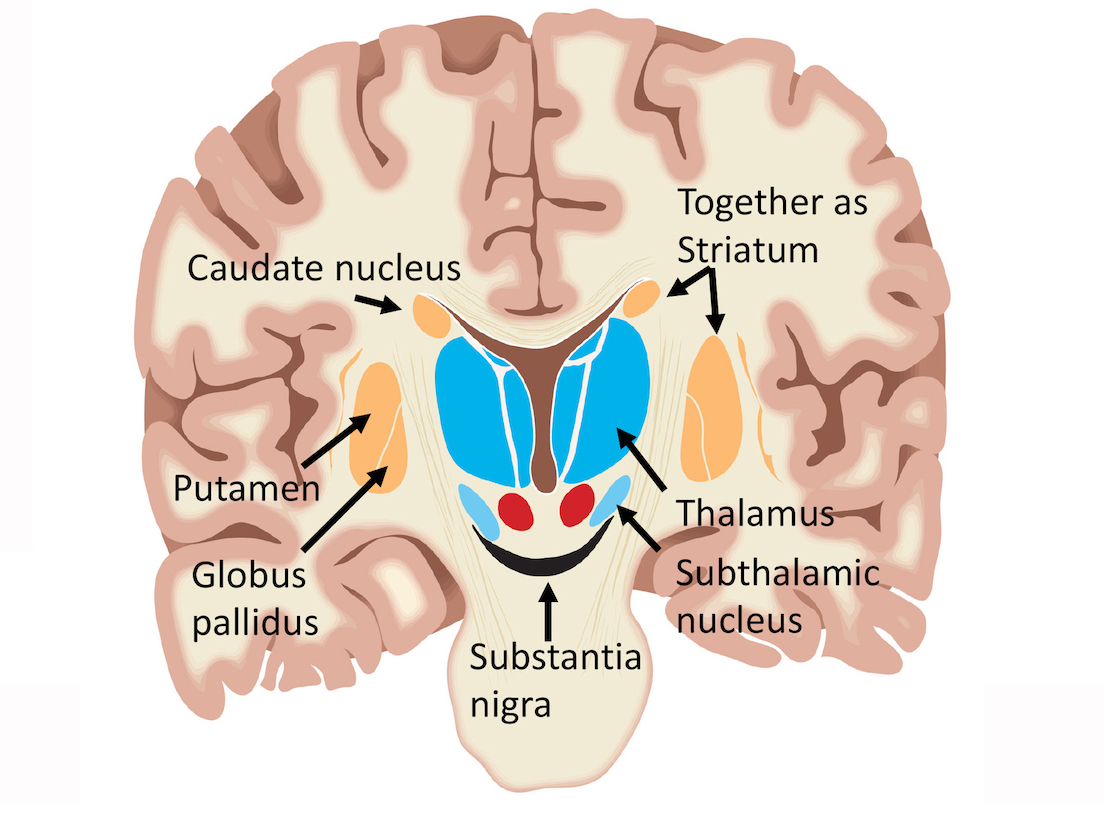
\includegraphics[scale=.3]{Images/bgnuclei.jpg}
    \caption{Artistic representation of the fundamental nuclei in the Basal Ganglia complex. (Figure adapted from \cite{bgnuclei}).}
    \label{fig:bgnuclei}
\end{figure}

\newpage
\subsection*{A higher degree of complexity}
So far the description of the connectivity in the Basal Ganglia brought out a complex network with a certain --- low, indeed --- degree of complexity. In reality, recent studies showed a much more intricate and complex connectivity among the BG nuclei. 
\\ One of the most important finding is the inclusion of the \emph{Cerebellum} in the Cortico-Basal Ganglia-Thalamocortical network. It has been found that the Cerebellum, specifically the \emph{Dentate nuclei} part of it, is connected to the SNr and the GPi. These connections are intriguing considering the also newly-found Cortico-Pallidal and Cortico-Nigral connections \cite{milardi}.
\\ A detailed figure showing all the recently newly found connections among Basal Ganglia nuclei can be found in \cite{simonyan}:

\begin{figure}[ht!]
    \centering
    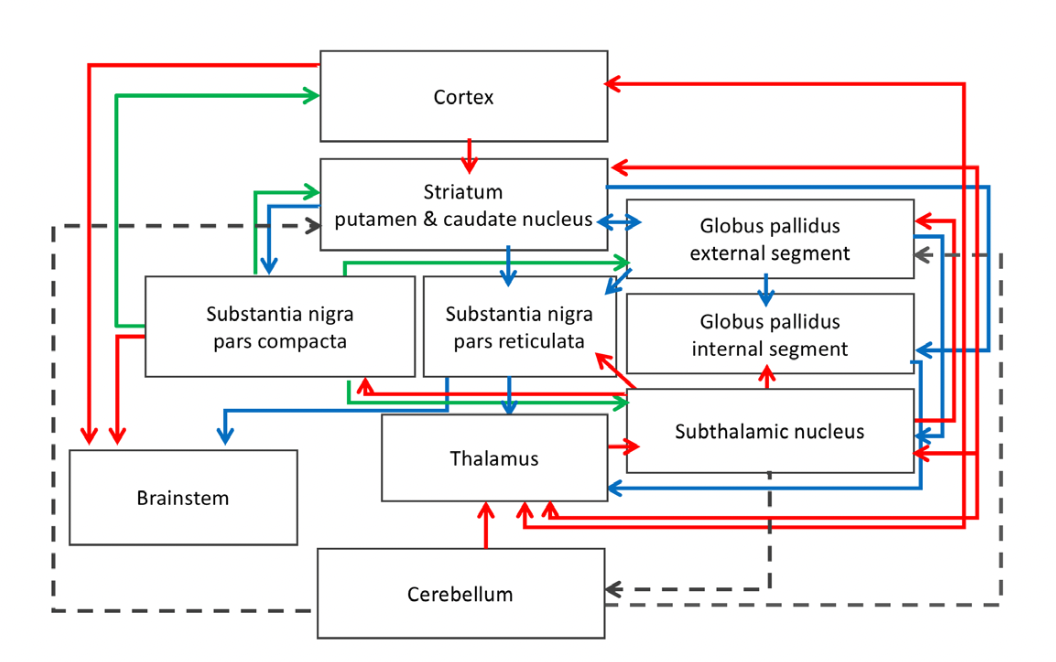
\includegraphics[scale=.8]{Images/network}
    \caption{Schematic representation of Basal Ganglia intrinsic and extrinsic connectivity.}
    \label{fig:network}
\end{figure}


\newpage
\subsection{Physiology}
%\ I pattern funzionali


\newpage
\section{Momevent disorders: a link with the Basal Ganglia}
%\ Iperkinesia --> Tourette // Ipokinesia --> Parkinson
%\ Cosa viene trovato in queste patologie a livello neurologico

\newpage
\section{Oscillapathies in the brain}

\newpage
\section{Deep Brain Stimulation: an empirical treatment}
%\ DBS come oscillatore Montgomery
\subsection{Open Loop}
\subsection{Closed Loop}

\newpage
\section{Oscillators in Physics}
\subsection{The Kuramoto Model}
\subsection{An extension: the Kuramoto-Sakaguchi model}

\newpage
\chapter{Methods and materials}


\bibliographystyle{unsrt}
\bibliography{biblio}
\end{document}